Over the various flow regimes; effusive, intermediate, and supersonic, the forward velocity and distributions change drastically from $\sim$100 m/s up to 800 m/s. We first consider the edge cases of the effusive and supersonic regimes. In the effusive regime, we make the assumption that the particles in the cell are non-interacting. We may rewrite the equation \ref{eq: mb_distribution} as a function of the mean velocity $\bar{v}$ into a simpler form,
\begin{equation}
	f(v) = \frac{32}{\pi^2} \frac{v^2}{\bar{v}^3} e^{-4v^2/\pi \bar{v}^2}. \label{eq: mb_simplified}
\end{equation}
To get the velocity distribution in the beam, we can calculate the distribution of particles incident on an aperture in the cell as
\begin{align*}
	f_{beam}(v) & = \frac{v}{\bar{v}}f(v)  \\
	& = \frac{32}{\pi^2} \frac{v^3}{\bar{v}^4} e^{-4v^2/\pi \bar{v}^2}.
\end{align*}
For low Reynold's numbers (Re<1) the flow at the aperture is purely molecular, which means that there are few to no collisions. This allows us to continue to use the Maxwell-Boltzmann distribution to describe the forward velocity \cite{Hutzler2011c},
\begin{equation}
	\bar{v}_\parallel = \int_0^\infty v f(v) dv \approx 1.2 \bar{v}.
\end{equation}
The spread of the forward velocity of an effusive beam is the full width half max (FWHM) of the Maxwell-Boltzmann distribution: $\Delta\bar{v} \approx 1.5 \bar{v}$. As the Reynolds number increases, one can reach the supersonic regime (Re>100) where the forward velocity reaches $1.4\bar{v}$ and the distribution drastically narrows.\cite{Hutzler2011c,Pauly}

The intermediate regime in between the effusive and supersonic regimes is particularly difficult to model, for there are some collisions at the aperture unlike the effusive regime, causing some boosting and narrowing, but not enough to treat the behavior as fully fluid-like. The section \ref{sec: beam density} results show that we can produce a beam in this intermediate regime by demonstrating clear hydrodynamic entrainment.

To better understand the reaction temperatures we will be able to reach, we need a characterization of the beam's velocity, more specifically, the velocity of the target species entrained within the buffer gas. The ideal target species is one with a reliable loading method and can be directly detected in small amounts. Ytterbium metal is known to have good ablation properties and the produced neutral isotopes have well known spectra. By ablating ytterbium foil inside of the experimental cell while the neon gas is being introduced, the ytterbium is cooled by the buffer gas and carried out of the cell. As long as the target species number density is a trace amount in comparison to the bulk buffer gas number density ($\leq$0.1\%), the flow characteristics are dominated by the buffer gas species \cite{Hutzler2012}. Based upon the results of our direct RGA measurements of the beam density, we know that the cell parameters used in the previous measurement land us in the intermediate flow regime due to the clear evidence of hydrodynamic entrainment.

To determine the velocity of the beam, we ablate an ytterbium target mounted inside the experimental cell where both neon and water are being introduced. The resulting beam is then illuminated with a 399 nm laser to excited the Yb. The laser is scanned over 3.5 GHz, encompassing all possible Yb isotope transitions. Two scans were taken, one with the 399 nm light perpendicular to the beam path (transverse), and the other where the laser is coming in with an angle of $\theta=57.3^\circ$ shown in Figure \ref{fig: Yb interrogation}. The resulting spectra are then fitted with summed Gaussian functions with predetermined isotopic shifts taken from literature, giving us the center (\ce{^174Yb}) frequency, as well as the thermally broadened width of the lines. Between the transverse and angled scans, we find an offset in the spectrum caused by the doppler shift, seen in figure \ref{fig: yb spectrum},
\begin{equation}
	\Delta f = \frac{\Delta v}{v} f \cos(\theta).
	\label{eq: doppler}
\end{equation}
Where $f$ is the fundamental center frequency, $\Delta f$ is the offset observed, $v$ is the forward velocity of the excited \ce{^174Yb}, and $\theta$ is the angle of the beam with respect to the beam. The fitted shared widths give us a beam temperature of 20 K, which is exactly what the experimental cell was held to. Using equation \ref{eq: doppler}, we find the forward velocity of the beam is around 150 m/s, in good agreement with a mildly boosted neon buffer gas of equilibrium temperature 20 K. 

\begin{figure}[H]
	\centering
	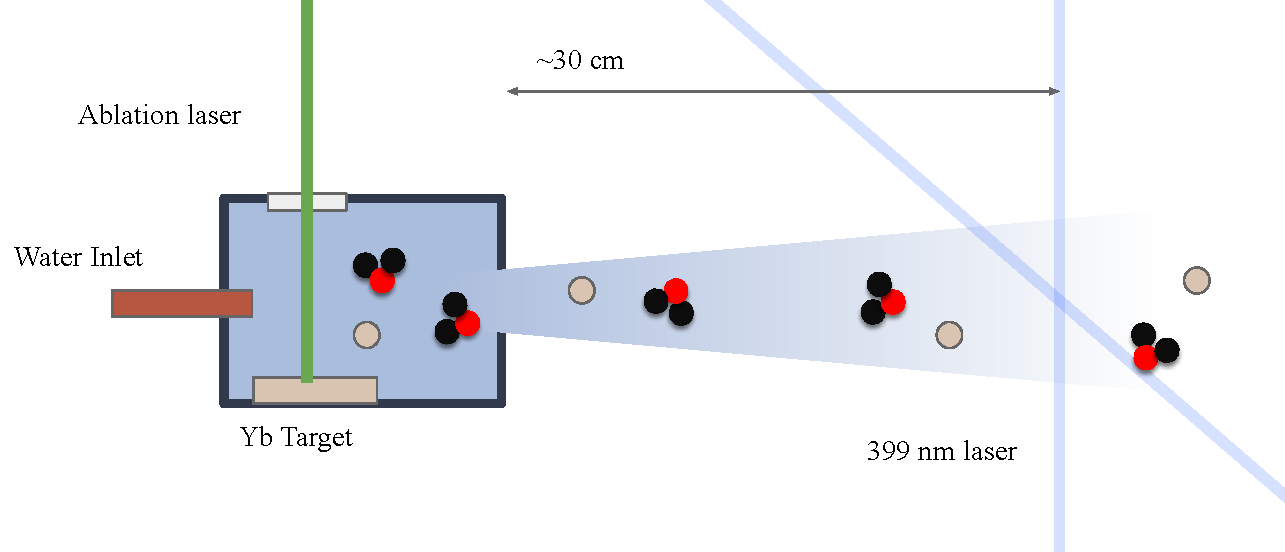
\includegraphics[width=\textwidth]{images/Yb_interrogation.pdf}
	\caption{Diagram of entrained neutral Yb interrogation where \ce{H2O} and Yb are entrained in a buffer gas of neon. The 399 nm laser is scanned over 3 GHz, recording the Yb isotope transitions both transverse, and at a 57.3$^\circ$ angle, to the beam.}
	\label{fig: Yb interrogation}
\end{figure}

%\begin{figure}[H]
%	\centering
%	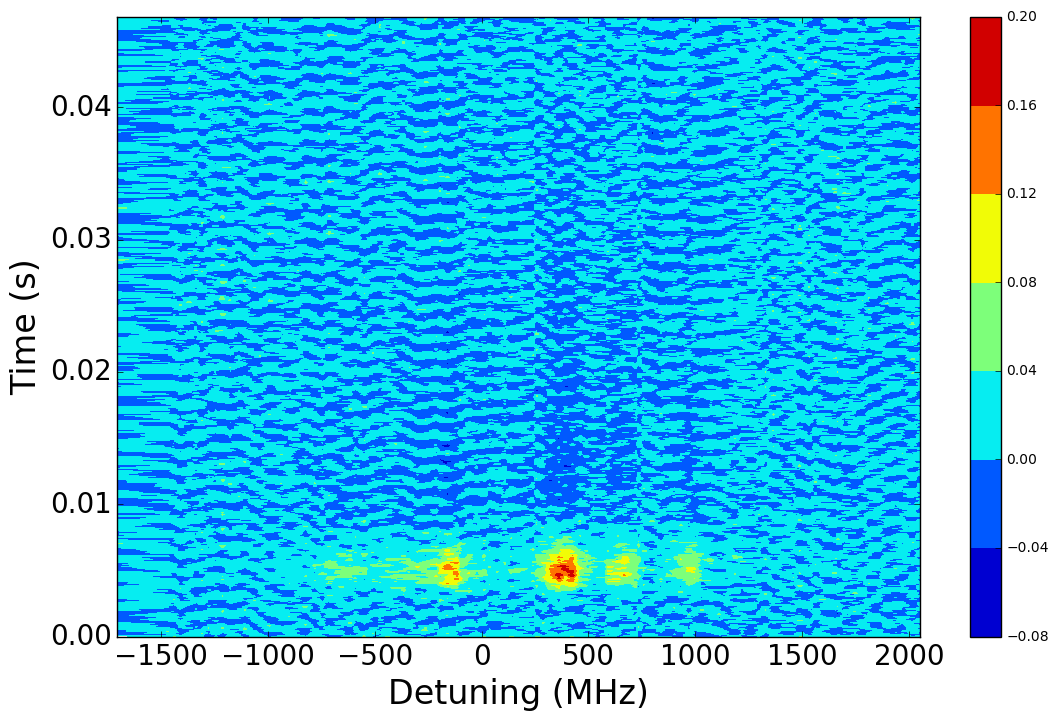
\includegraphics[width=1\textwidth]{images/CBGB_Yb_spectrum_scan.png}
%	\caption{}
%	\label{fig: yb_spectrum_scan}
%\end{figure}

\begin{figure}[H]
	\centering
	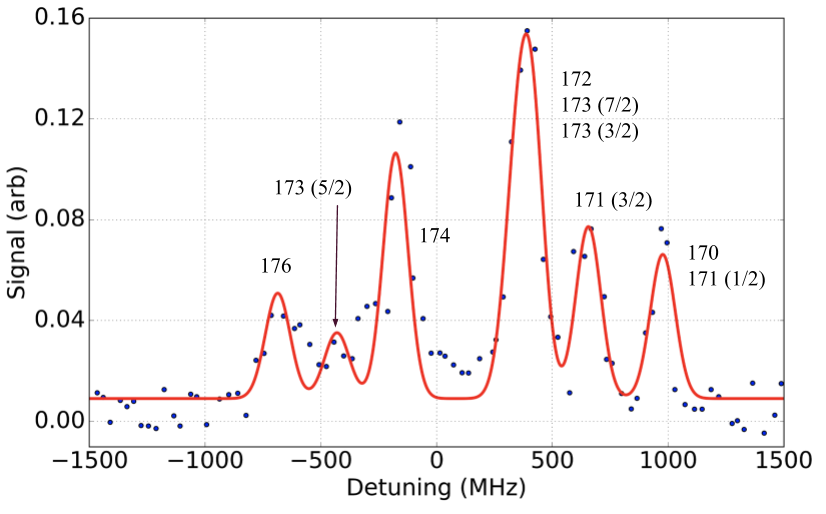
\includegraphics[width=0.8\textwidth]{images/CBGB_Yb_spectrum_long_labeled.png}
	\caption{Angled longitudinal scan of Yb fluorescence collected by PMT at $\approx 24$ cm from cell aperture offset relative to the measured \ce{^174Yb} frequency from a transverse scan. A fit of Gaussians on the observed Yb isotopic transitions is shown with fixed detunings, while shared widths and individual heights are kept free fitting parameters. Fits yield a forward velocity of $\approx 150$ m/s and broadened width of 20 K.}
	\label{fig: yb spectrum}
\end{figure}

We find that the Yb is entrained within the neon and sympathetically cooled to the cell's temperature. The water that is also introduced in the beam will also be at a similar temperature and forward velocity as long as the neon density is much larger than that of the water when the beam dynamics is dominated by the properties of the buffer gas species.
